\documentclass[11pt]{report}
% PACKAGES
  \usepackage[a4paper,left=28mm,right=28mm,top=30mm,bottom=30mm]{geometry}
  \usepackage{graphicx,epstopdf}      % Used to import external graphics (figures)
  \usepackage{hyperref}       % Used for referring to links inside and outside the document
  \usepackage[table]{xcolor}  % To include colors 
  \usepackage{amsmath}        % For most of the math symbols and environments (such as \begin{align})
  \usepackage{amssymb}        % For using symbols in the document
  \usepackage{float}          % Arranging of figures on the page
  \usepackage[bf]{caption}    % Arranging the captions in floating environments [bf] makes the Figures bold
  \usepackage{subcaption}     % To arrange captions of subfigures
  \usepackage{booktabs}       % For standard tabular tables, with rules
  \usepackage{tabularx}       % For clean tables such as in the Nomenclature
  \usepackage{fancyhdr}       % Fancy headers
  % \usepackage[colorinlistoftodos]{todonotes}      % To create todo notes
  \usepackage[nottoc,notlot,notlof]{tocbibind}    % Add bibliography to content
  \usepackage{bm}             % Make bold symbols
  \usepackage{lipsum}
  \usepackage{parskip}
  \usepackage[export]{adjustbox}
  \usepackage{changepage}
% LAY-OUT
  % \usepackage{pdfpages}

  % \usepackage{pdflscape}

   \renewcommand\thesection{\arabic{section}}

  % \usepackage[mathletters]{ucs}
  % \usepackage[utf8x]{inputenc}
  %Bibliography for references, with reference style options
  \usepackage[
  backend=biber,
  bibstyle=ieee,
  citestyle=numeric-comp,
  dashed=false,
  url = false,
  maxnames=8,
  maxcitenames=2,
  mincitenames=1,
  sorting=none,
  isbn = false,
  doi = false
  ]{biblatex}
  \addbibresource{references.bib}

  %Set the page style
  \pagestyle{fancy}
  \fancyhead[L]{\ifodd\value{page} \slshape\nouppercase{\rightmark} \else \fi}
  \fancyhead[R]{\ifodd\value{page} \else \slshape\nouppercase{\leftmark} \fi}
  \chead{ }
  \lfoot{}
  \rfoot{}
  \cfoot{\small\thepage}


  %Give colors to links/refs etc
  \hypersetup{colorlinks, linkcolor={blue!0!black}, 
                          citecolor={blue!70!black}, 
                           urlcolor={blue!80!}} 
                       
  %% Set up numbering and spacing
  \numberwithin{equation}{section}        %Number the equations per section
  \numberwithin{figure}{section}          %Number the figures per section
  \numberwithin{table}{section}           %Number the tables per section
  \captionsetup[table]{skip=1pt}          %Skip 1 pt after a table
  \captionsetup[figure]{skip=3.5pt}       %Skip 4 pt after a figure
  \setcounter{secnumdepth}{3}             %Count up to the subsubsection 
  \setcounter{topnumber}{1}               %Number of floats at top of a page (default is 2)

  %%%%% proof/theorem/definition boxes

  \usepackage{cleveref}
  \usepackage[most]{tcolorbox}
  \newtcbtheorem{Theorem}{Theorem}{
    enhanced,
    sharp corners,
    attach boxed title to top left={
      yshifttext=-1mm
    },
    colback=white,
    colframe=blue!75!black,
    fonttitle=\bfseries,
    boxed title style={
      sharp corners,
      size=small,
      colback=blue!75!black,
      colframe=blue!75!black,
    } 
  }{thm}

  \newtcbtheorem{Definition}{Definition}{
    enhanced,
    sharp corners,
    attach boxed title to top left={
      yshifttext=-1mm
    },
    colback=white,
    colframe=blue!25,
    fonttitle=\bfseries,
    coltitle=black,
    boxed title style={
      sharp corners,
      size=small,
      colback=blue!25,
      colframe=blue!25,
    } 
  }{def}

  \newtcbtheorem[no counter]{Proof}{Proof}{
    enhanced,
    sharp corners,
    attach boxed title to top left={
      yshifttext=-1mm
    },
    colback=white,
    colframe=blue!25,
    fonttitle=\bfseries,
    coltitle=black,
    boxed title style={
      sharp corners,
      size=small,
      colback=blue!25,
      colframe=blue!25,
    } 
  }{prf}
% DEFINITIONS
  %% Titlepage definitions
  \newcommand{\deltitle}{Impact-Aware Control for a Dual-Arm Setup}      %Your project title
  \newcommand{\StudentName}{Gijs van den Brandt}  %Student name
  \newcommand{\StudentID}{1257110}                    %Your student number
  % \newcommand{\DCcode}{2021.109}                      %Get your DC code from the D&C secretariat

  %% Operators
  \DeclareMathOperator\sign{sgn}                      %Sign function
  \DeclareMathOperator\diag{diag}                     %Diagonal operator
  \DeclareMathOperator\imag{Imag}                     %Imaginary part of complex variable
  \DeclareMathOperator\real{Real}                     %Real part of complex variable
  \DeclareMathOperator*{\argmin}{\arg\!\min}          %Argmin operator
  \newcommand{\norm}[1]{\left\lVert#1\right\rVert}    %Norm operator

  %% Variable definition
  \newcommand{\R}{\mathbb{R}}                         % Set of real numbers
  \newcommand{\C}{\mathbb{C}}                         % Set of complex numbers

\begin{document}
\section*{Nomenclature}

$\begin{array}{l}
\text{\textbf{Joint space}}\\
q \;\quad \text{Joint positions}\\
M \;\quad \text{Inertia matrix}\\
\\
\text{\textbf{Posture task space}}\\
\beta \quad \text{Desired acceleration of the first joint } q_1\\
k \;\quad \text{Posture stiffness}\\

\\
\text{\textbf{Impedance task space} (all variables are expressed in world frame)}\\
R \quad \text{Rotation matrix of the end effector}\\
\omega \quad \text{Angular velocity vector of the end effector}\\
\alpha \quad \text{Angular acceleration vector of the end effector}\\
p \;\quad \text{Position vector of the end effector}\\
v \;\quad \text{Linear velocity vector of the end effector}\\
a \;\quad \text{Linear acceleration vector of the end effector}\\
f \;\quad \text{Virtual wrench vector acting on the end effector}\\
K \quad \text{Impedance stiffness matrix} \\
\Lambda \;\quad \text{Impedance inertia matrix} \\
\\

\text{\textbf{Reference Spreading}}\\
\varphi  \quad \text{Time of impact}\\
\Delta \varphi \; \text{Offset between measured impact and reference extension}\\
\gamma  \quad \text{Normalized time since impact}\\
T  \quad \text{Duration of interim impact mode}\\
m \quad \text{RS mode selector (-1: no RS, 
0: no interim, 1: Jari, 2: Sven, 3: mixing)}\\
j \quad \text{Number of jumps that have occured}\\\\
\text{\textbf{Sub- and superscripts}}\\
(\cdot)_{dem} \quad \text{Signals from VR device during recording}\\
(\cdot)_{rec} \;\quad \text{Signals measured from robot or calculated during recording}\\
(\cdot)_{ext} \;\quad \text{Signals resulting from the splitting and extending of the recorded signal}\\
(\cdot)_{ref} \;\quad \text{Signals determined using RS scheme}\\
(\cdot)_{rep} \;\quad \text{Signals measured from robot or calculated during replay}\\
\end{array}$
\newpage
\section*{Recording}

$\begin{array}{l}
\ddot{q}_{rec} = \min\limits_{\ddot{q}}\left \|  \begin{bmatrix}
\alpha(\ddot{q})\\ 
a(\ddot{q})
\end{bmatrix} - \Lambda^{-1}f_{rec} \right \| + \left \| \ddot{q}_1-\beta_{rec} \right \|\\\\
f_{rec} =2(\Lambda K_{rec})^{\frac{1}{2}} \begin{bmatrix}
\omega_{dem} - \omega_{rec}
\\ 
v_{dem}-v_{rec}
\end{bmatrix} + K_{rec} \begin{bmatrix}
R_{rec}(\log({R_{rec}}^TR_{dem}))^{\vee }\\ 
p_{dem}-p_{rec}
\end{bmatrix}\\\\
\beta_{rec} = 2\sqrt{k_{rec}}\left [ -\dot{q}_{1,rec}  \right ] + k_{rec}\left [ -q_{1,rec}  \right ]

\end{array}$\\
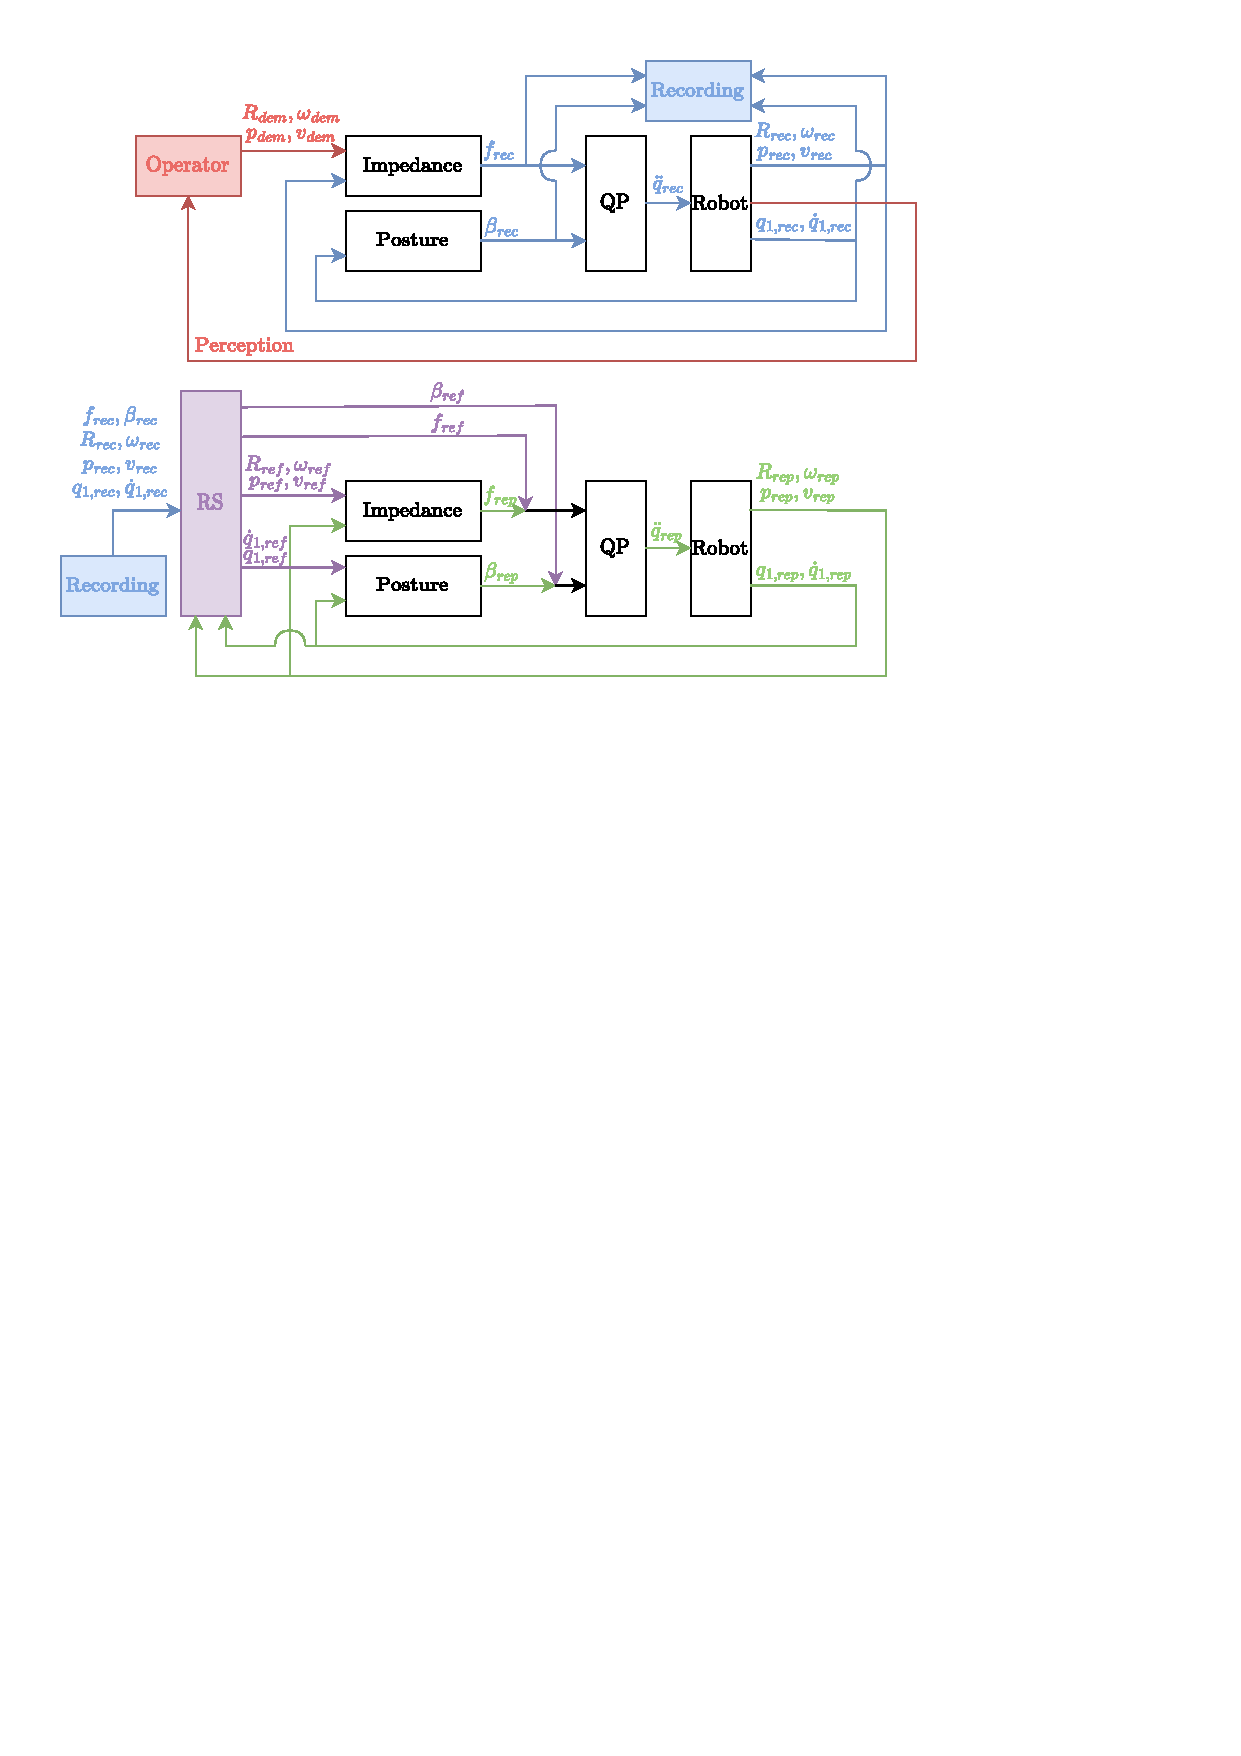
\includegraphics[trim={1cm 23.3cm 5cm 1cm}, clip]{Graphics/qp.pdf}\\

\section*{Replaying}
$\begin{array}{l}
\ddot{q}_{rep} = \min\limits_{\ddot{q}}\left \|  \begin{bmatrix}
\alpha(\ddot{q})\\ 
a(\ddot{q})
\end{bmatrix} - \Lambda^{-1}(f_{rep}+f_{ref}) \right \| + \left \|\ddot{q}_1-(\beta_{rep}+\beta_{ref}) \right \|\\\\
f_{rep} =2(\Lambda K_{rep})^{\frac{1}{2}} \begin{bmatrix}
\omega_{ref} - \omega_{rep}
\\ 
v_{ref}-v_{rep}
\end{bmatrix} + K_{rep} \begin{bmatrix}
R_{rep}(\log({R_{rep}}^TR_{ref}))^{\vee }\\ 
p_{ref}-p_{rep}
\end{bmatrix}\\\\
\beta_{rep} = 2\sqrt{k_{rep}}\left [ \dot{q}_{1,ref}-\dot{q}_{1,rep}  \right ] + k_{rep}\left [ q_{1,ref}-q_{1,rep}  \right ]
\end{array}$

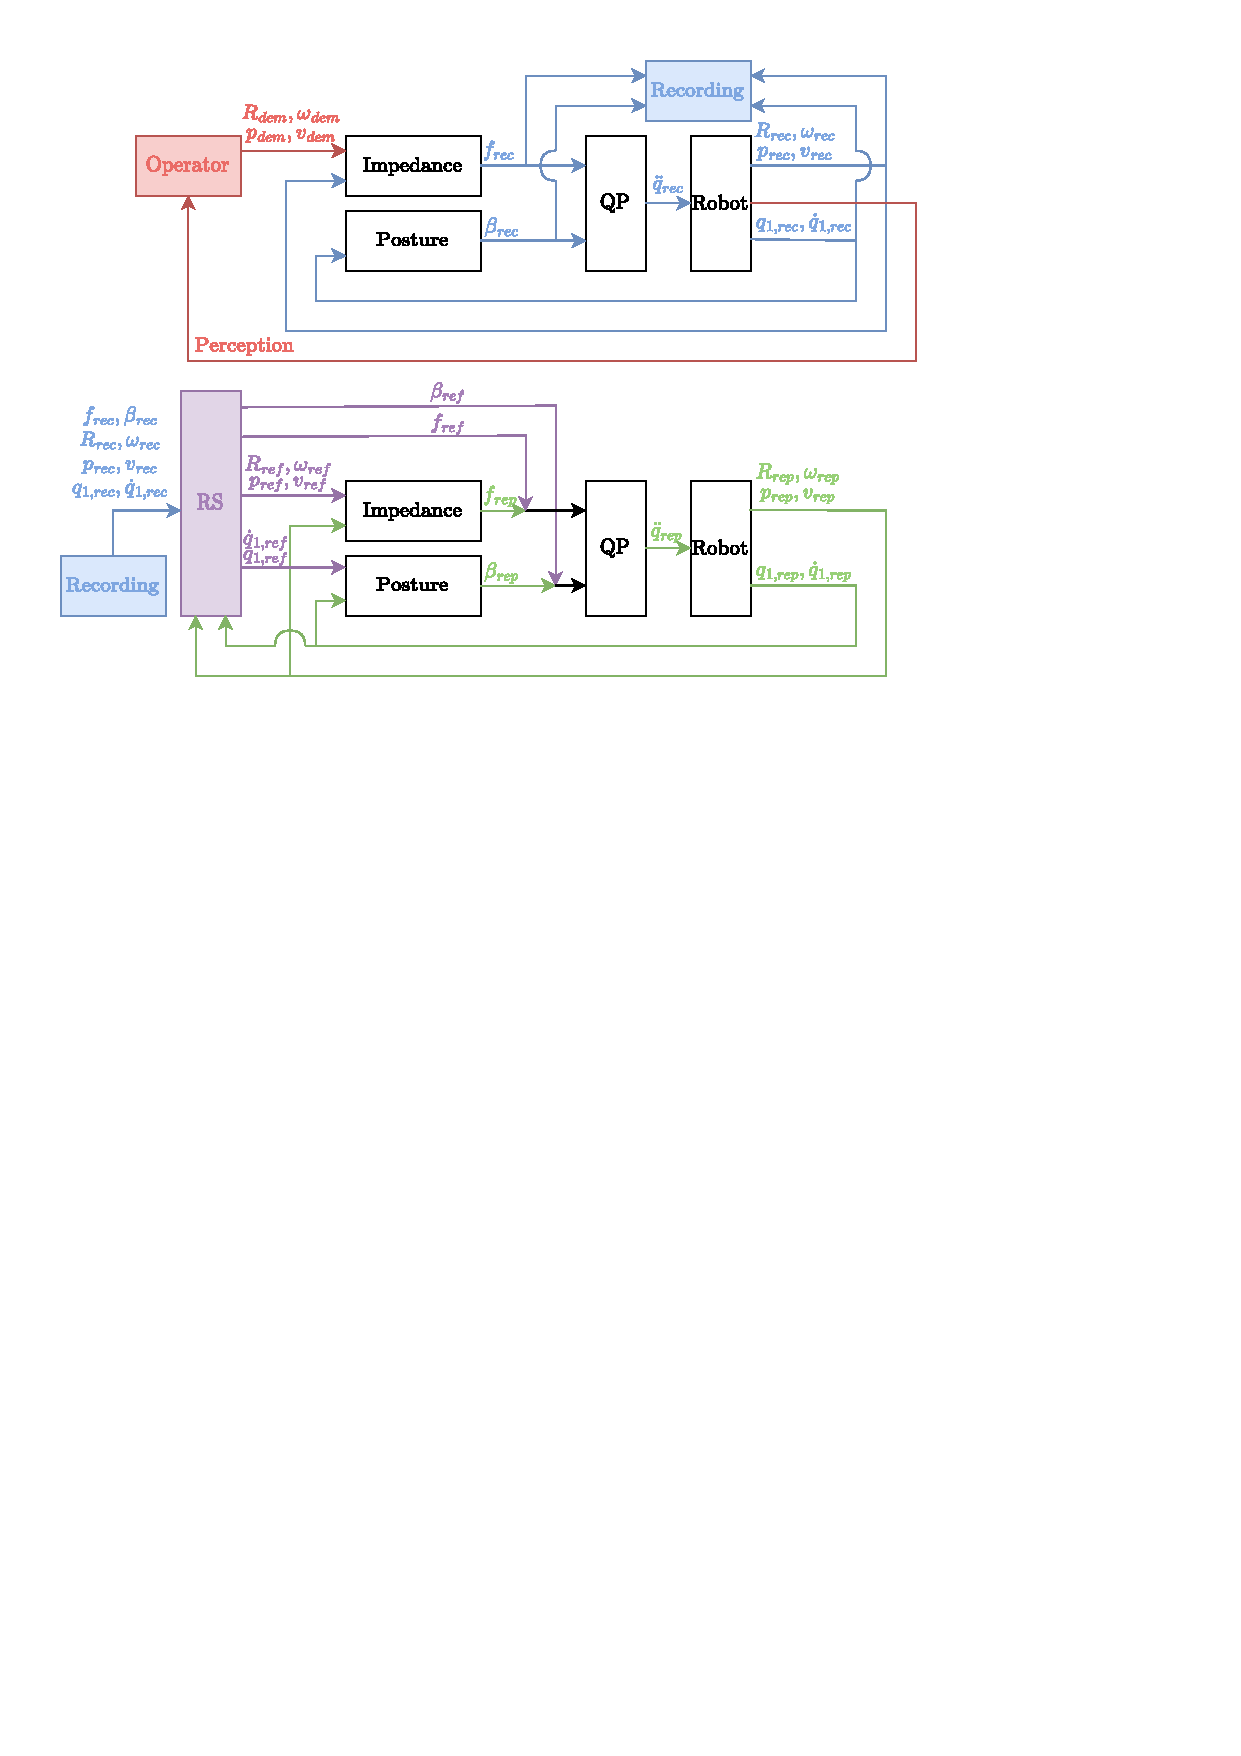
\includegraphics[trim={1cm 17.8cm 5cm 6.5cm}, clip]{Graphics/qp.pdf}
\\
\section*{Reference Extending}
$\begin{array}{l}

$$\varphi_{rec}^- = \varphi_{rec}(j)+\Delta \varphi$$\\
$$\varphi_{rec}^+ = \varphi_{rec}(j+1)-\Delta \varphi$$\\
\\
$$\Omega = \begin{bmatrix}
0 & -\omega_3 & \omega_2\\ 
\omega_3 & 0 &-\omega_1 \\ 
 -\omega_2 & \omega_1 & 0
\end{bmatrix}$$\\
\\
S_{hold}(x) 
= \begin{cases} 
x(\varphi_{rec}^-),& \text{if } t< \varphi_{rec}^-\\
x(\varphi_{rec}^+),& \text{if } t> \varphi_{rec}^+\\
x(t) ,& \text{otherwise}\\
\end{cases}\\
\\

S_{integ}(x,y) 
= S_{hold}(x)+\begin{cases} 
y(\varphi_{rec}^-)(t-\varphi_{rec}^+),& \text{if } t< \varphi_{rec}^-\\
y(\varphi_{rec}^+)(t-\varphi_{rec,j}^-),& \text{if } t> \varphi_{rec}^+\\
0 ,& \text{otherwise}\\
\end{cases}\\
\\

S_{rot}(R,\omega) 
= \begin{cases} 
R(\varphi_{rec}^-)e^{\Omega(\varphi_{rec}^-)(t-\varphi_{rec}^-)},& \text{if } t< \varphi_{rec}^-\\
R(\varphi_{rec}^+)e^{\Omega(\varphi_{rec}^+)(t-\varphi_{rec}^+)},& \text{if } t> \varphi_{rec}^+\\
R(t) ,& \text{otherwise}\\
\end{cases}\\
\\

\\

R_{ext,j}(t,j) = S_{rot}(R_{rec}(t),\omega_{rec}(t))\\

\\
\begin{bmatrix} 
p_{ext,j}(t,j)  \\
 q_{1,ext,j}(t,j) 
\end{bmatrix} = S_{integ} \left (
\begin{bmatrix} 
p_{rec}(t)\\
 q_{1,rec}(t)
\end{bmatrix} 
,\begin{bmatrix} 
v_{rec}(t)\\
 \dot{q}_{1,rec}(t)
\end{bmatrix} 
 \right )\\
\\

\\
\begin{bmatrix} 
\omega_{rec}(t,j)\\
v_{ext}(t,j)\\
 \dot{q}_{1,ext}(t,j)\\
 f_{ext}(t,j)\\
 \beta_{ext}(t,j)
\end{bmatrix} = S_{hold} \left (
\begin{bmatrix} 
\omega_{rec}(t)\\
v_{rec}(t)\\
 \dot{q}_{1,rec}(t)\\
 f_{rec}(t)\\
 \beta_{rec}(t)
\end{bmatrix}
\right )\\
\\

\end{array}$

Note that the functions $S_{hold}$, $S_{integ}$, and $S_{rot}$ also require $\varphi_{rec}$ to be evaluated. This dependancy is excluded from notation for brevity. 
\section*{Reference Switching}

$\begin{array}{l}
\gamma = \frac{t-\varphi_{rep,j}}{T}\\

U_{jump}(x_{rep},x_{ext}) = \begin{cases} 
x_{ext}(t,j_{rec}),& \text{if } m = -1\\
x_{ext}(t,j_{rep}),& \text{if } m = 0\\
x_{ext}(t,j_{rep}),& \text{if } (\gamma \geq 1)\wedge (m \notin \{ -1,0 \} )\\
x_{ext}(t,j_{rep}),& \text{if } (\gamma < 1)\wedge(m=0)\\ 
x,& \text{if } (\gamma < 1)\wedge(m=1)\\ 
0,& \text{if } (\gamma < 1)\wedge(m=2)\\ 
\gamma x_{ext}(t,j_{rep}) ,& \text{if } (\gamma < 1)\wedge(m=3)\\ \end{cases}\\\\
\\

U_{cont}(x_{ext}) = \begin{cases} 
x_{ext}(t,j_{rec}),& \text{if } m = -1\\
x_{ext}(t,j_{rep}),& \text{if } m = 0\\
x_{ext}(t,j_{rep}),& \text{if } (\gamma \geq 1)\wedge (m \notin \{ -1,0 \} )\\
x_{ext}(t,j_{rep}) ,& \text{if } (\gamma < 1)\wedge(m=0)\\ 
x_{ext}(t,j_{rep}-1) ,& \text{if } (\gamma < 1)\wedge(m=1)\\ 
x_{ext}(t,j_{rep}-1) ,& \text{if } (\gamma < 1)\wedge(m=2)\\ 
\gamma x_{ext}(t,j_{rep})+ (1-\gamma)x_{ext}(t,j_{rep}-1) ,& \text{if } (\gamma < 1)\wedge(m=3)\\ \end{cases}\\\\\\
\\


U_{cont}(R_{ext}) = \begin{cases} 
R_{ext}(t,j_{rec}),& \text{if } m = -1\\
R_{ext}(t,j_{rep}),& \text{if } m = 0\\
R_{ext}(t,j_{rep}),& \text{if } (\gamma \geq 1)\wedge (m \notin \{ -1,0 \} )\\
R_{ext}(t,j_{rep}) ,& \text{if } (\gamma < 1)\wedge(m=0)\\ 
R_{ext}(t,j_{rep}-1) ,& \text{if } (\gamma < 1)\wedge(m=1)\\ 
R_{ext}(t,j_{rep}-1) ,& \text{if } (\gamma < 1)\wedge(m=2)\\ 
R_{ext}(t,j_{rep}-1)(R^T_{ext}(t,j_{rep}-1)R_{ext}(t,j_{rep}))^\gamma ,& \text{if } (\gamma < 1)\wedge(m=3)\\ \end{cases}\\\\\\

R_{ref}(t) = U_{rot}(R_{ext}(t,j))\\

\\
\begin{bmatrix} 
p_{ref}(t) \\
 q_{1,ref}(t) \\
 f_{ref}(t)\\
 \beta_{ref}(t)
\end{bmatrix} = U_{cont} \left (
\begin{bmatrix} 
p_{ext}(t,j)\\
 f_{ext}(t,j)\\
 \beta_{ext}(t,j)
\end{bmatrix} 
 \right )\\
\\

\\
\begin{bmatrix} 
\omega_{ref}(t)\\
v_{ref}(t)\\
 \dot{q}_{1,ref}(t,j)\\
\end{bmatrix} = U_{jump} \left (

\begin{bmatrix} 
\omega_{rep}(t)\\
v_{rep}(t)\\
 \dot{q}_{1,rep}(t)\\
\end{bmatrix},

\begin{bmatrix} 
\omega_{ext}(t,j)\\
v_{ext}(t,j)\\
 \dot{q}_{1,ext}(t,j)\\
\end{bmatrix}

\right )\\
\\
\end{array}$
Note that the functions $U_{jump}$, $U_{cont}$, and $U_{rot}$ also require $j_{rep}$, $j_{rec}$, $\gamma$ and $m$ to be evaluated. These dependencies are excluded from notation for brevity. 
\newpage

\section*{Miscelaneous}
$\begin{array}{l}
\begin{bmatrix}
\omega\\ 
v
\end{bmatrix} = J\dot{q}\\\\
\begin{bmatrix}
\alpha(\ddot{q})\\ 
a(\ddot{q})
\end{bmatrix} = J\ddot{q} + \dot{J}\dot{q}\\\\
\Lambda^{-1} = J^TM^{-1}J
\end{array}$

Need a different symbol for $\dot{q}_1$ since it is not always the derivative of $q_1$. 
\end{document}